% mnras_template.tex
%
% LaTeX template for creating an MNRAS paper
%
% v3.0 released 14 May 2015
% (version numbers match those of mnras.cls)
%
% Copyright (C) Royal Astronomical Society 2015
% Authors:
% Keith T. Smith (Royal Astronomical Society)

% Change log
%
% v3.0 May 2015
%    Renamed to match the new package name
%    Version number matches mnras.cls
%    A few minor tweaks to wording
% v1.0 September 2013
%    Beta testing only - never publicly released
%    First version: a simple (ish) template for creating an MNRAS paper

%%%%%%%%%%%%%%%%%%%%%%%%%%%%%%%%%%%%%%%%%%%%%%%%%%
% Basic setup. Most papers should leave these options alone.
\documentclass[a4paper,fleqn,usenatbib]{mnras}

% MNRAS is set in Times font. If you don't have this installed (most LaTeX
% installations will be fine) or prefer the old Computer Modern fonts, comment
% out the following line
\usepackage{newtxtext,newtxmath}
% Depending on your LaTeX fonts installation, you might get better results with one of these:
%\usepackage{mathptmx}
%\usepackage{txfonts}

% Use vector fonts, so it zooms properly in on-screen viewing software
% Don't change these lines unless you know what you are doing
\usepackage[T1]{fontenc}
\usepackage{ae,aecompl}

%%%%% AUTHORS - PLACE YOUR OWN PACKAGES HERE %%%%%

% Only include extra packages if you really need them. Common packages are:
\usepackage{graphicx}	% Including figure files
\usepackage{amsmath}	% Advanced maths commands
\usepackage{amssymb}	% Extra maths symbols
\usepackage[xindy]{glossaries}

%%%%%%%%%%%%%%%%%%%%%%%%%%%%%%%%%%%%%%%%%%%%%%%%%%

%%%%% AUTHORS - PLACE YOUR OWN COMMANDS HERE %%%%%

% Please keep new commands to a minimum, and use \newcommand not \def to avoid
% overwriting existing commands. Example:
%\newcommand{\pcm}{\,cm$^{-2}$}	% per cm-squared

\newcommand{\GSF}[1]{\noindent\textcolor{blue}{GSF:#1}}

%glossary
\newacronym{alfa}{ALFA}{Arecibo L-Band Feed Array}
\newacronym{dm}{DM}{Dispersion Measure}
\newacronym{frb}{FRB}{Fast Radio Burst}
\newacronym{fwhm}{FWHM}{Full-Width at Half-Maximum}
\newacronym{gbt}{GBT}{Greenbank Telescope}
\newacronym{if}{IF}{Intermediate Frequency}
\newacronym{igm}{IGM}{Intergalactic Medium}
\newacronym{ism}{ISM}{Interstellar Medium}
\newacronym{nip}{NIP}{Non-image Processing}
\newacronym{pll}{PLL}{Phased-locked Loop}
\newacronym{rfi}{RFI}{Radio-frequency Interference}
\newacronym{ska}{SKA}{Square Kilometre Array}
\newacronym{sefd}{SEFD}{System Equivalent Flux Density}
\newacronym{snr}{SNR}{Signal-to-Noise Ratio}
\newacronym{sps}{SPS}{Single Pulse Search}

%%%%%%%%%%%%%%%%%%%%%%%%%%%%%%%%%%%%%%%%%%%%%%%%%%

% Title of the paper, and the short title which is used in the headers.
% Keep the title short and informative.
\title[Verification Tests for FRB Detections]{Verification Tests for FRB
Detections}

\author[ALFABURST Team]{
ALFABURST Team
}
%% The list of authors, and the short list which is used in the headers.
%% If you need two or more lines of authors, add an extra line using \newauthor
%\author[K. T. Smith et al.]{
%Keith T. Smith,$^{1}$\thanks{E-mail: mn@ras.org.uk (KTS)}
%A. N. Other,$^{2}$
%Third Author$^{2,3}$
%and Fourth Author$^{3}$
%\\
%% List of institutions
%$^{1}$Royal Astronomical Society, Burlington House, Piccadilly, London W1J 0BQ, UK\\
%$^{2}$Department, Institution, Street Address, City Postal Code, Country\\
%$^{3}$Another Department, Different Institution, Street Address, City Postal Code, Country
%}

% These dates will be filled out by the publisher
\date{Accepted XXX. Received YYY; in original form ZZZ}

% Enter the current year, for the copyright statements etc.
\pubyear{2017}

% Don't change these lines
\begin{document}
\label{firstpage}
\pagerange{\pageref{firstpage}--\pageref{lastpage}}
\maketitle

% Abstract of the paper
\begin{abstract}
% What is the point of the paper?
% What is the context of the study? What background information is necessary to understand the study?
% How was the study done?
% What is the main take away message?
% What can be said about these results, and how does this affect future work?
The ALFABURST commensal FRB survey has been in operation since June 2015. In
that time a number of false-positive events, which on initial inspect appear to
be FRB-like, have been found to be of local origin. Here we report on one such event
as an example of the difficult challenge of fully automating an FRB search. The
one-off nature of most FRBs requires extra scrutiny in reporting an
astrophysical FRB and triggering automated follow-ups with a telescope network.
\end{abstract}

% Select between one and six entries from the list of approved keywords.
% Don't make up new ones.
\begin{keywords}
radio continuum: transients -- methods: observational
\end{keywords}

%%%%%%%%%%%%%%%%% BODY OF PAPER %%%%%%%%%%%%%%%%%%

% TODO: notebook of dec 4 event, low SNR event, make filterbanks available

\section{Introduction}
\label{sec:intro}

Over two years of the initial ALFABURST survey over 125k 8-second windows have
been recorded in which our \gls{frb} search pipeline detected an event above the
minimum \gls{snr} detection threshold. The vast majority of these events have been
due to \gls{rfi}, some of the events are due bright single pulses of known
pulsars. Sorting through these false positive events is the main focus of our
post-processing methods. Most of the events are clearly \gls{rfi} which are
classified with an automated classifier model. A small number of windows contain
FRB-like events which only on further inspection of the data, the telescope
operation status, and contextual information is it clear that these events are
from local sources.

\section{Example: A dispersed pulse}
\label{sec:D20161204}

A narrow-in-time, broad-in-frequency, millisecond pulse was detected with the
ALFABURST \citep{2017ApJS..228...21C} system at MJD 57726.563263913 / Unix time
1480858266 (09:31:06 Arecibo local time) in Beam 0 (the central beam) of the
\gls{alfa} receiver (Figure \ref{fig:beam0_dynamic_spec}). ALFABURST was
processing 56 MHz of bandwidth between 1457 MHz and 1513 MHz. The \gls{snr} of
this pulse is maximized (10.46) when the pulse is dedispersed with a \gls{dm} of
293 and the 256 microsecond resolution is decimated by a factor of 16 to 4 ms
time resolution. We believe this event to have been generated by a local source,
mostly likely within the receiver dome.
%
% notebooks/event_figures.ipynb
\begin{figure}
    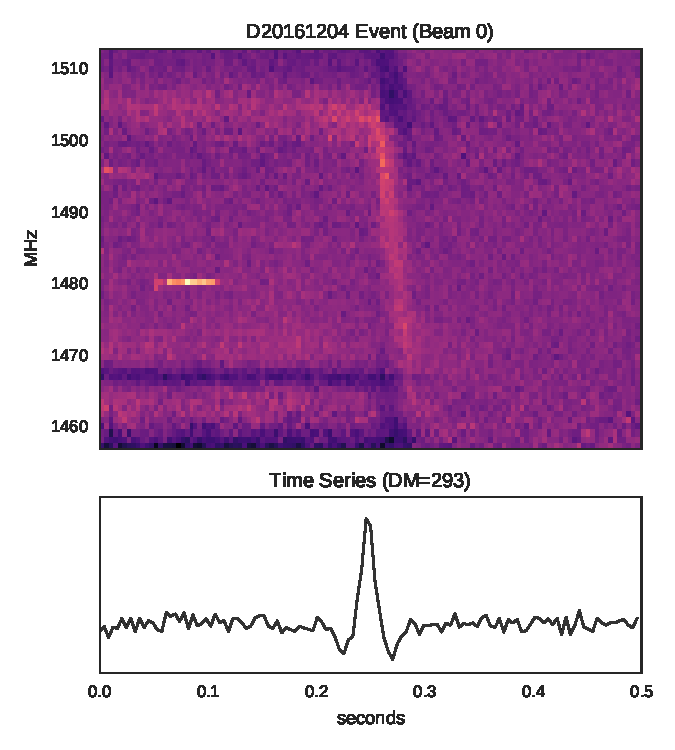
\includegraphics[width=1.0\linewidth]{figures/D20161204_buf23_Beam0.pdf}
    \caption{Dynamic spectrum (top) and dedispersed time series (bottom) of an
    FRB-like event that was detected in beam 0 of the ALFA receiver on December
    4, 2016. The dynamic spectrum has been bandpass normalized. The
    characteristic dip before and after the event is due to zero-DM removal
    which is part of the ALFABURST RFI exciser. The strong, narrowband source at
    1480 MHz around 0.1 s is due to a  local RFI source.
    }
    \label{fig:beam0_dynamic_spec}
\end{figure}
%
The flux density of the event can be computed with the radiometer equation
%
$$
S = \textrm{SEFD} \frac{\textrm{SNR}}{\sqrt{D \; \Delta \tau \;
\Delta \nu}}
$$
%
using an \gls{sefd} of 3 Jy for the \gls{alfa} receiver. This results in a flux
density of $S = 66$ mJy from Beam 0, which would be lower flux than any
previously detected \gls{frb} \citep{2016PASA...33...45P}. Flux estimate is an
upper limit, as we are assuming the source was at the centre of the beam.

In isolation this pulse looks like a potential \gls{frb}. A bright \gls{frb} can
show up in multiple \gls{alfa} beams, so we inspected all other events in the
same time window as the Beam 0 event. An event was found in Beam 5 only. This
pulse lines up exactly in time with the Beam 0 event but the \gls{frb} was
maximized (15.99) with a DM=829 dedispersion. Upon further inspection and
testing different DMs for dedispersion we found that this event appeared to
narrow in width at lower DM. We see that there was \gls{rfi} clipping in this
event which is known to introduce a bias. This could account for the increased
DM to maximize the SNR. The Beam 0 and Beam 5 event are the same event. The
higher \gls{snr} and \gls{rfi} clipping in Beam 5 indicates that the signal was
stronger in that beam.

But, the Beam 5 spectrogram introduces new issues with this event being an
non-terrestrial \gls{frb}. Before and after the event there are events that look
similar to the main event, these event SNRs are maximized by choosing a range of
DMs.

Further, there is a serious red flag when inspecting the bandpass during the
event. The detection band of \gls{alfa} was chosen because it is the most
sensitive region of the band, and relatively flat. But during the event there is
a noticeable shape and slant to the bandpass which is not seen in a typical
observation (Figure \ref{fig:bandpass_response}). The system noise appears
higher, which could indicate an introduction of a stable, warm source to the
system. There is also narrow-in-frequency, periodic RFI at 1468, 1480, 1496,
1504 MHz not usually seen in this band. In the high time and frequency
resolution view these short pulses in 12.5 MHz steps have a characteristic
dampened harmonic oscillation due to frequency locking with a \gls{pll} (Figure
\ref{fig:pll_spectrum}).
%
% notebooks/event_figures.ipynb
\begin{figure}
    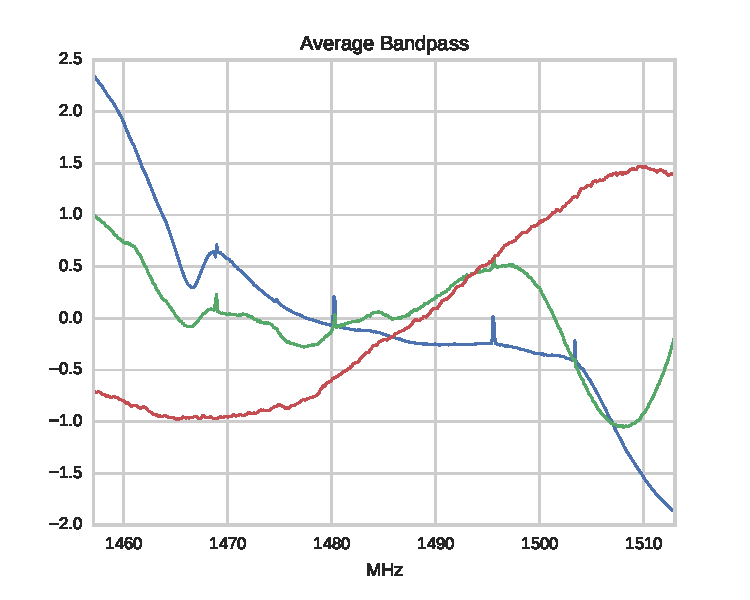
\includegraphics[width=1.0\linewidth]{figures/bandpass_response.pdf}
    \caption{Average bandpass response during the Decmber 4, 2016 event for beam
    0 (green) and beam 5 (blue). A typical bandpass (red) is plotted for
    reference. These bandpasses have been normalized in the detection pipeline.
    }
    \label{fig:bandpass_response}
\end{figure}
%

%
% notebooks/event_figures.ipynb
\begin{figure}
    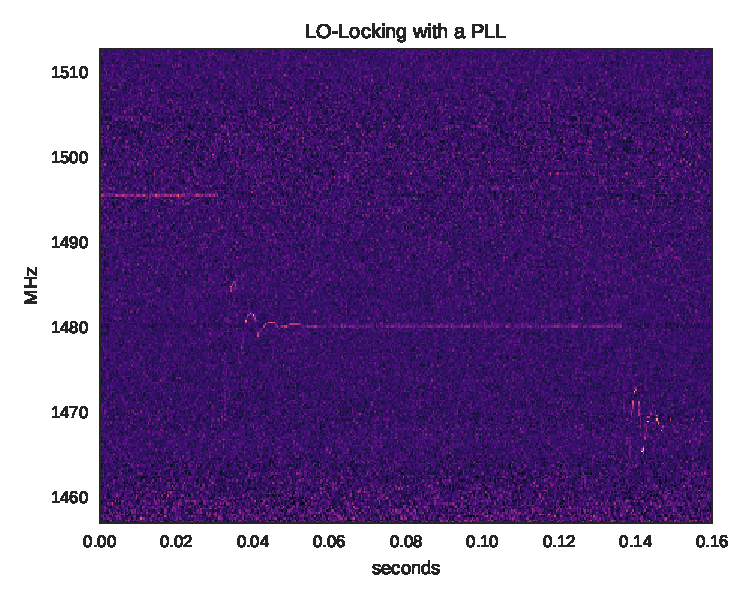
\includegraphics[width=1.0\linewidth]{figures/pll_spectrum.pdf}
    \caption{Dynamic spectrum when a local oscialltor in the receiver dome is
    being locked with a phased-locked loop circuit. This LO is not related to
    the receiver analogue mixing chain, but rather it is associated with RFI
    monnitoring equipment.
    }
    \label{fig:pll_spectrum}
\end{figure}
%

We considered that the band could have been changed. We have setup the automated
system to restart observations when the \gls{if} frequency is changed. The
Arecibo telescope logging data is reported locally in SCRAM packets which
provide pointing, frequency tuning, and receiver information at approximately
one second resoltuion. During the time of the event there was no change in the
\gls{if} during that time and the telescope was pointed at a fixed Dec
(+15:11:28.34) and drifting in RA (event detected at RA=14:42:26.18), i.e. a
fixed (alt,az) pointing.

Looking at the observation schedule for the morning of December 4, project P3080
was using \gls{alfa} to perform an \gls{frb} survey of the Virgo cluster until
09:00 local time. From there Project R3037 was scheduled, this is an S-Band
RADAR observation. \gls{alfa} was not register as switched off until around
10:00, approximately 15 minutes after the event was detected. This indicated to
us that the events we are seeing all likely related to the setup of the S-Band
RADAR.

% TODO: dec 4 event: turret in wrong position

Looking at a longer time window before the event we found further indication of
time and frequency-variable structure in the band before the event which looks
related. Approximately 90 seconds before the event we see the band change in
multiple beams, and the appearance of narrow-in-frequency \gls{rfi}.

Currently, we are considering that the event is due to ALFA being covered to
protect against the RADAR system while it was still the active rx. It could be
that this event is due to some standing-wave coupling between the ALFA and the
cover.

% TODO: What is the physical process which generated this event?
% TODO: explanation of terrestial FRB detection
% TODO: follow-up to verify is is a local source, what is the source?

In isolation, and the one-off, transient nature of FRBs make the initial Beam 0
detection look very reasonable. It is only with an extended study of the
meta-data, earlier-in-time evolution of the band, and use of multiple beams to
confirm that this is indeed not an FRB.

\section{Verification Checks}

% TODO:
% low SNR events, due to sudden changes in the noise statistics, expect to
% detect a few of these based in the minimum SNR, what is the time scale for an
% SNR 6 event? these events are due to turrent movement, add flag to filter out
% figure: DM - t plot

% TODO:
% decision tree
% important tests:
%   bandpass check
%   telescope status
%   negative DM statistics
%   previous in time events

% TODO: DM search space: 0-10000, no negative DMs, could reveal RFI by comparing
%  number of events detected in positive and negative DM search space

% TODO: considerations for automated follow-up/VOevents

% TODO: considerations for releasing FRB event data as they are one-off events that
% require extra scrutiny

% TODO:
% future developments in FRB surveys require additional layers of processing.
% large surveys will produce an abundance of false positives. it is cumbersome
% to follow up events now. in the future it will be impossible. additional
% layers should prioritize events by how interesting they are

\bibliographystyle{mnras}
\bibliography{../alfaburst.bib} 

% Don't change these lines
\bsp	% typesetting comment
\label{lastpage}
\end{document}

% End of mnras_template.tex
